% LBEADS-NET Thesis Defense Presentation
% Saad Zubairi — NYU Tandon — May 2026
\documentclass[aspectratio=169, 10pt]{beamer}

% ─────────────────────────────────────────────
% Packages
% ─────────────────────────────────────────────
\usepackage[utf8]{inputenc}
\usepackage[T1]{fontenc}
\usepackage{amsmath,amssymb,bm}
\usepackage{tikz}
\usetikzlibrary{arrows.meta, positioning, calc, decorations.pathmorphing, shapes.geometric, fit, backgrounds}
\usepackage{pgfplots}
\pgfplotsset{compat=1.18}
\usepackage{tcolorbox}
\tcbuselibrary{skins, breakable}
\usepackage{booktabs}
\usepackage{appendixnumberbeamer}
\usepackage{graphicx}
\usepackage{pifont}% for ding marks

% ─────────────────────────────────────────────
% Theme Setup
% ─────────────────────────────────────────────
\usetheme{metropolis}
\setbeamertemplate{navigation symbols}{}
\setbeamertemplate{footline}[frame number]

% Color Palette
\definecolor{navy}{HTML}{1A365D}
\definecolor{steelblue}{HTML}{2B6CB0}
\definecolor{forestgreen}{HTML}{276749}
\definecolor{warningred}{HTML}{C53030}
\definecolor{lightgray}{HTML}{F7FAFC}
\definecolor{midgray}{HTML}{E2E8F0}

\setbeamercolor{palette primary}{bg=navy, fg=white}
\setbeamercolor{frametitle}{bg=navy, fg=white}
\setbeamercolor{title}{fg=navy}
\setbeamercolor{alerted text}{fg=warningred}
\setbeamercolor{example text}{fg=forestgreen}
\setbeamercolor{block title}{bg=steelblue, fg=white}
\setbeamercolor{block body}{bg=lightgray}

% tcolorbox styles
\newtcolorbox{resultgood}{colback=forestgreen!8, colframe=forestgreen, fonttitle=\bfseries, title={}}
\newtcolorbox{resultbad}{colback=warningred!8, colframe=warningred, fonttitle=\bfseries, title={}}
\newtcolorbox{insightbox}{colback=steelblue!8, colframe=steelblue, fonttitle=\bfseries, title={}}

% Checkmark / crossmark
\newcommand{\cmark}{\textcolor{forestgreen}{\ding{51}}}
\newcommand{\xmark}{\textcolor{warningred}{\ding{55}}}
\newcommand{\wmark}{\textcolor{orange}{\ding{115}}}

% ─────────────────────────────────────────────
% Title Information
% ─────────────────────────────────────────────
\title{LBEADS-NET}
\subtitle{Algorithm Unrolling for Learned Baseline Estimation\\and Denoising in Chromatographic Signals\\[0.5em]\small MS Thesis Defense}
\author{Saad Zubairi\\[0.3em]{\small Advisor: Professor Ivan Selesnick}}
\institute{New York University\\Tandon School of Engineering}
\date{May 2026}

% ─────────────────────────────────────────────
\begin{document}

% =============================================
% SLIDE 1 — Title
% =============================================
\begin{frame}[plain]
  \maketitle
\end{frame}

% =============================================
% ACT I: THE PROBLEM (Slides 2–8)
% =============================================
\section{Act I: The Problem}

% =============================================
% SLIDE 2 — What is a Chromatogram?
% =============================================
\begin{frame}{What is a Chromatogram?}
\note{Chromatography separates chemical compounds. The detector records peaks whose areas are proportional to concentration. Baseline drift corrupts these measurements.}
\centering
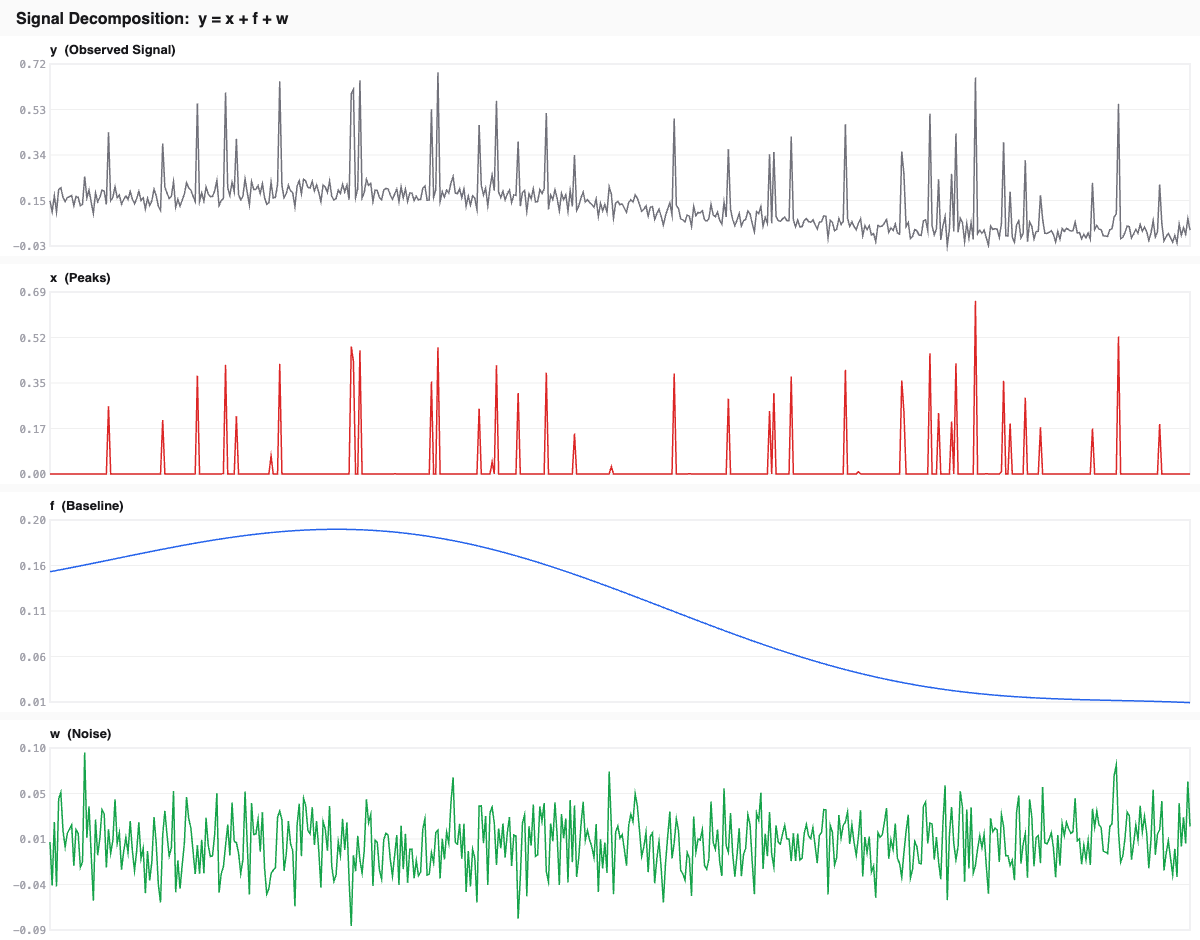
\includegraphics[width=0.75\textwidth, height=0.75\textheight, keepaspectratio]{figures/Signal_3_decomposition.png}

\vspace{0.3em}
\centering
\textcolor{navy}{\textbf{The observed signal is a mixture of three components:}} $\;\mathbf{y} = \mathbf{x} + \mathbf{f} + \mathbf{w}$
\end{frame}

% =============================================
% SLIDE 3 — Why Baseline Correction Matters
% =============================================
\begin{frame}{Why Baseline Correction Matters}
\begin{columns}[T]
\begin{column}{0.48\textwidth}
\centering
\textcolor{forestgreen}{\textbf{Correct Baseline}}

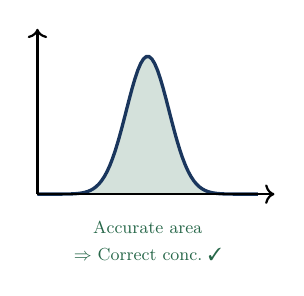
\begin{tikzpicture}[scale=0.7, transform shape]
  \fill[forestgreen!20, domain=0:4, samples=80]
    (0,0) -- plot (\x, {2.5*exp(-(\x-2)^2/0.3)}) -- (4,0) -- cycle;
  \draw[navy, very thick, domain=0:4, samples=80]
    plot (\x, {2.5*exp(-(\x-2)^2/0.3)});
  \draw[forestgreen, thick, dashed] (0,0) -- (4,0);
  \draw[->, thick] (0,0) -- (4.3,0);
  \draw[->, thick] (0,0) -- (0,3);
  \node[forestgreen] at (2, -0.6) {\small Accurate area};
  \node[forestgreen] at (2, -1.1) {\small $\Rightarrow$ Correct conc.\ \cmark};
\end{tikzpicture}
\end{column}

\begin{column}{0.48\textwidth}
\centering
\textcolor{warningred}{\textbf{Wrong Baseline}}

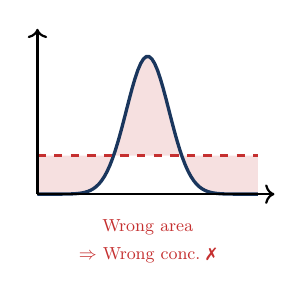
\begin{tikzpicture}[scale=0.7, transform shape]
  \fill[warningred!15, domain=0:4, samples=80]
    (0,0.7) -- plot (\x, {2.5*exp(-(\x-2)^2/0.3)}) -- (4,0.7) -- cycle;
  \draw[navy, very thick, domain=0:4, samples=80]
    plot (\x, {2.5*exp(-(\x-2)^2/0.3)});
  \draw[warningred, thick, dashed] (0,0.7) -- (4,0.7);
  \draw[->, thick] (0,0) -- (4.3,0);
  \draw[->, thick] (0,0) -- (0,3);
  \node[warningred] at (2, -0.6) {\small Wrong area};
  \node[warningred] at (2, -1.1) {\small $\Rightarrow$ Wrong conc.\ \xmark};
\end{tikzpicture}
\end{column}
\end{columns}

\vspace{1em}
\begin{insightbox}
In pharmaceutical QC, even 2\% baseline error can exceed regulatory limits.
\end{insightbox}
\end{frame}

% =============================================
% SLIDE 4 — The Classical Solution: BEADS
% =============================================
\begin{frame}{The Classical Solution: BEADS}
\textbf{B}aseline \textbf{E}stimation \textbf{A}nd \textbf{D}enoising using \textbf{S}parsity \hfill{\scriptsize (Ning et al., 2014)}

\vspace{0.5em}
\begin{equation*}
J(\mathbf{x}) = \tfrac{1}{2}\|H(\mathbf{y} - \mathbf{x})\|_2^2 + \lambda_0 \sum_n \theta(x_n) + \lambda_1 \sum_n \phi(\Delta x_n) + \lambda_2 \sum_n \phi(\Delta^2 x_n)
\end{equation*}

\vspace{0.5em}
\begin{enumerate}
  \item \textcolor{steelblue}{\textbf{Data fidelity}} — high-pass filter $H$ separates baseline from peaks
  \item \textcolor{steelblue}{\textbf{Asymmetric sparsity penalty}} $\theta$ — peaks are sparse and non-negative
  \item \textcolor{steelblue}{\textbf{First-order smoothness}} — penalizes peak roughness
  \item \textcolor{steelblue}{\textbf{Second-order smoothness}} — penalizes peak curvature
\end{enumerate}

\vspace{0.8em}
\begin{resultbad}
\centering
\textbf{6 parameters to tune:} $\;\lambda_0,\;\lambda_1,\;\lambda_2,\;r,\;f_c,\;d$
\end{resultbad}
\end{frame}

% =============================================
% SLIDE 5 — The Tuning Problem
% =============================================
\begin{frame}{The Tuning Problem}
\centering
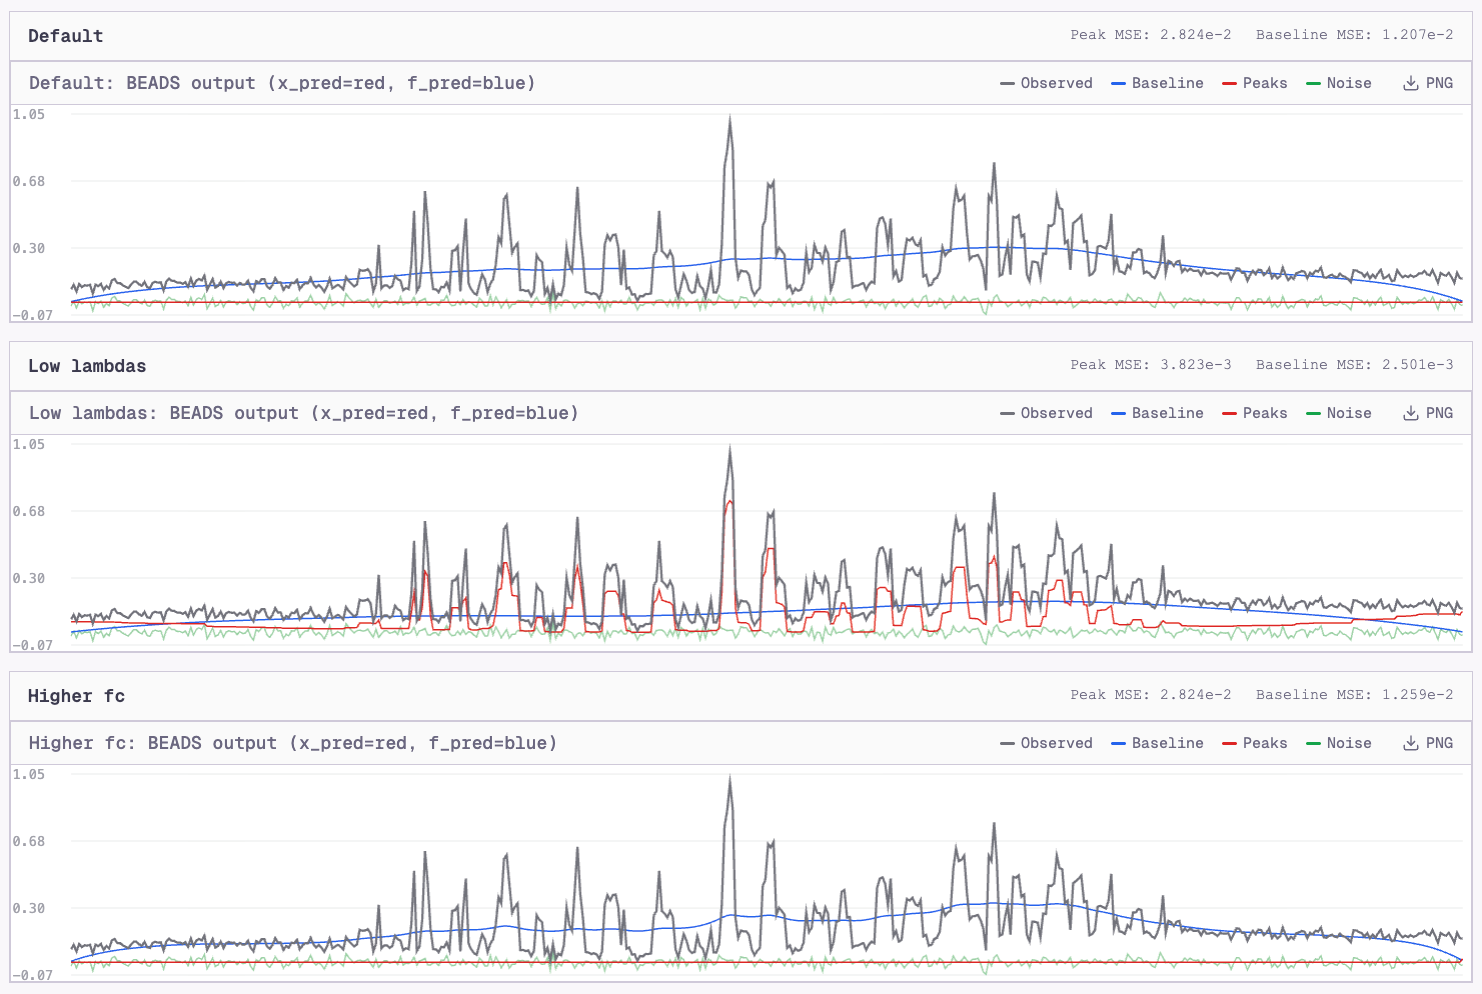
\includegraphics[width=0.85\textwidth, height=0.65\textheight, keepaspectratio]{figures/BEADS_EXAMPLE.png}

\vspace{0.8em}
\begin{resultbad}
\centering
\textbf{No single parameter configuration generalizes across instruments, analytes, or conditions.}
\end{resultbad}
\end{frame}

% =============================================
% SLIDE 6 — The Deep Learning Alternative
% =============================================
\begin{frame}{The Deep Learning Alternative}
\begin{itemize}
  \setlength\itemsep{0.7em}
  \item \textbf{Convolutional autoencoders} (Kensert et al., 2021) --- 190K synthetic chromatograms
  \item \textbf{ResUNet} (Chen et al., 2022) --- 2.35M parameters, 210K spectra
  \item \textbf{DIRAS+} (Aradhye et al., 2025) --- hybrid CNN + classical solver
\end{itemize}

\vspace{0.8em}
These methods generalize without per-signal tuning\ldots

\vspace{0.5em}
\begin{resultbad}
\centering
\ldots but they are \textbf{black boxes} with millions of opaque parameters.
\end{resultbad}
\end{frame}

% =============================================
% SLIDE 7 — The Gap
% =============================================
\begin{frame}{The Gap}
\centering
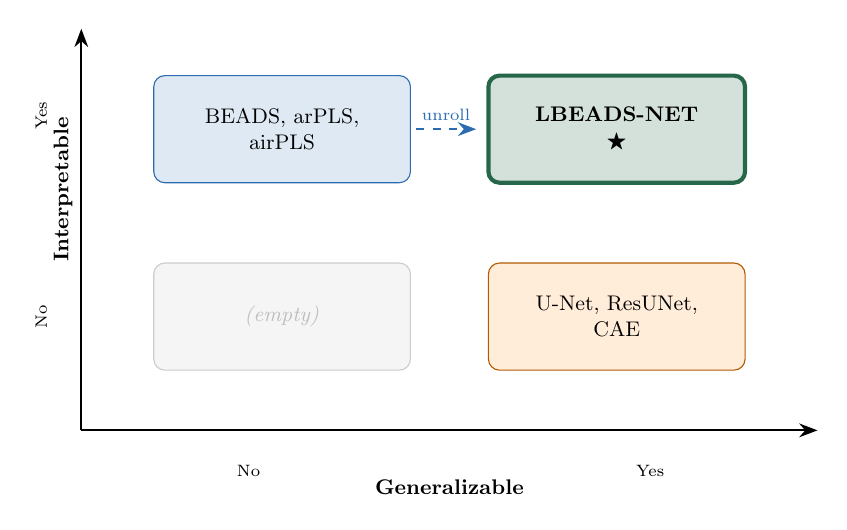
\begin{tikzpicture}[
    box/.style={minimum width=3.8cm, minimum height=1.6cm, rounded corners=4pt, align=center, text width=3.6cm, font=\small},
    scale=0.85, transform shape
  ]
  % Axes
  \draw[-{Stealth}, thick] (-0.5, -0.5) -- (10.5, -0.5) node[midway, below=0.6cm, font=\small\bfseries] {Generalizable};
  \draw[-{Stealth}, thick] (-0.5, -0.5) -- (-0.5, 5.5) node[midway, above=0.6cm, rotate=90, font=\small\bfseries] {Interpretable};

  \node[font=\scriptsize] at (2, -1.1) {No};
  \node[font=\scriptsize] at (8, -1.1) {Yes};
  \node[font=\scriptsize, rotate=90] at (-1.1, 1.2) {No};
  \node[font=\scriptsize, rotate=90] at (-1.1, 4.2) {Yes};

  % Top-left: Classical
  \node[box, fill=steelblue!15, draw=steelblue] at (2.5, 4) {BEADS, arPLS,\\airPLS};

  % Bottom-right: Deep Learning
  \node[box, fill=orange!15, draw=orange!70!black] at (7.5, 1.2) {U-Net, ResUNet,\\CAE};

  % Bottom-left: empty
  \node[box, fill=gray!8, draw=gray!40, text=gray!50] at (2.5, 1.2) {\textit{(empty)}};

  % Top-right: LBEADS-NET (starred)
  \node[box, fill=forestgreen!20, draw=forestgreen, line width=1.5pt] (lbeads) at (7.5, 4) {\textbf{LBEADS-NET}\\$\bigstar$};

  % Arrow
  \draw[-{Stealth}, thick, dashed, steelblue] (4.5, 4) -- (5.4, 4) node[midway, above, font=\scriptsize] {unroll};
\end{tikzpicture}
\end{frame}

% =============================================
% SLIDE 8 — Our Approach: Algorithm Unrolling
% =============================================
\begin{frame}{Our Approach: Algorithm Unrolling}
\begin{columns}[T]
\begin{column}{0.42\textwidth}
\vspace{0.5em}
\begin{itemize}
  \setlength\itemsep{0.6em}
  \item Map each \textbf{iteration} of an optimization algorithm to one \textbf{neural network layer}
  \item Algorithm parameters $\rightarrow$ \textbf{learnable} network parameters
  \item $K$ layers = $K$ iterations, trained \textbf{end-to-end}
\end{itemize}

\vspace{0.8em}
\textcolor{navy}{\textbf{LBEADS-NET:}}

20 layers $\times$ 5 parameters = \textbf{100 learnable scalars}
\end{column}

\begin{column}{0.55\textwidth}
\centering
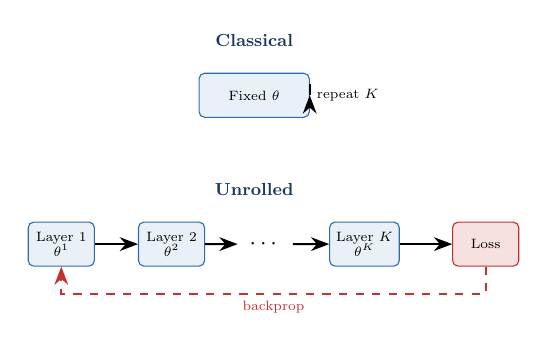
\begin{tikzpicture}[scale=0.7, transform shape,
    block/.style={rectangle, draw=steelblue, fill=steelblue!10, minimum width=1.2cm, minimum height=0.8cm, rounded corners=2pt, font=\scriptsize, align=center},
    arr/.style={-{Stealth}, thick}
  ]
  % Classical
  \node[font=\small\bfseries, text=navy] at (0, 4.5) {Classical};
  \node[block, minimum width=2cm] (cl) at (0, 3.5) {Fixed $\theta$};
  \draw[arr] (cl.east) to[out=30, in=-30, looseness=3] node[right, font=\scriptsize] {repeat $K$} (cl.east);

  % Unrolled
  \node[font=\small\bfseries, text=navy] at (0, 1.8) {Unrolled};
  \node[block] (l1) at (-3.5, 0.8) {Layer 1\\$\theta^1$};
  \node[block] (l2) at (-1.5, 0.8) {Layer 2\\$\theta^2$};
  \node[font=\large] at (0.2, 0.8) {$\cdots$};
  \node[block] (lk) at (2, 0.8) {Layer $K$\\$\theta^K$};
  \node[block, fill=warningred!15, draw=warningred] (loss) at (4.2, 0.8) {Loss};

  \draw[arr] (l1) -- (l2);
  \draw[arr] (l2) -- (-0.3, 0.8);
  \draw[arr] (0.7, 0.8) -- (lk);
  \draw[arr] (lk) -- (loss);
  \draw[arr, dashed, warningred] (loss.south) -- ++(0,-0.5) -| (l1.south) node[pos=0.25, below, font=\scriptsize, text=warningred] {backprop};
\end{tikzpicture}
\end{column}
\end{columns}
\end{frame}


% =============================================
% ACT II: THE ATTEMPT (Slides 9–21)
% =============================================
\section{Act II: The Attempt}

% =============================================
% SLIDE 9 — From BEADS to BEADSLayer
% =============================================
\begin{frame}{From BEADS to BEADSLayer}
\begin{columns}[T]
\begin{column}{0.45\textwidth}
\textcolor{steelblue}{\textbf{Classical BEADS (one iteration)}}
\vspace{0.3em}
\begin{enumerate}
  \setlength\itemsep{0.3em}
  \item Compute reweighting matrices $\Lambda, \Gamma$
  \item Assemble system matrix $M$
  \item Solve banded linear system\\$(B^\top\!B + A^\top\!MA)\,\mathbf{z} = \mathbf{d}$
  \item Update $\mathbf{x}^{(k+1)} = A\mathbf{z}$
\end{enumerate}
\end{column}

\begin{column}{0.08\textwidth}
\centering
\vspace{2cm}
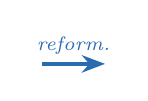
\begin{tikzpicture}
  \draw[-{Stealth}, very thick, steelblue] (0,0) -- (0.8,0);
  \node[above, font=\scriptsize\itshape, text=steelblue] at (0.4,0) {reform.};
\end{tikzpicture}
\end{column}

\begin{column}{0.45\textwidth}
\textcolor{forestgreen}{\textbf{ISTA Layer (one layer)}}
\vspace{0.3em}
\begin{enumerate}
  \setlength\itemsep{0.3em}
  \item Gradient step:\\
    $\mathbf{x}_{\text{up}} = \mathbf{x}^{k-1} + \eta\,\mathbf{g}_{\text{data}}$\\
    $\phantom{\mathbf{x}_{\text{up}}} - \eta(\nabla\!\mathcal{R}_1 + \nabla\!\mathcal{R}_2)$
  \item Proximal step:\\
    $\mathbf{x}^k = \mathcal{S}_{\text{asym}}(\mathbf{x}_{\text{up}};\;\lambda_0\eta,\;r)$
\end{enumerate}
\end{column}
\end{columns}

\vspace{1em}
\begin{insightbox}
Replace exact linear system solve with \textbf{gradient descent + proximal operator}.
\end{insightbox}
\end{frame}

% =============================================
% SLIDE 10 — The ISTA Layer
% =============================================
\begin{frame}{The ISTA Layer}
\textbf{Gradient step:}
\[
\mathbf{x}_{\text{update}} = \mathbf{x}^{k-1} + \eta^k \,\mathbf{g}_{\text{data}} - \eta^k\!\left(\nabla_{\mathbf{x}}\mathcal{R}_1 + \nabla_{\mathbf{x}}\mathcal{R}_2\right)
\]

\textbf{Proximal step} (asymmetric soft-thresholding):
\[
[\mathbf{x}^k]_i = \begin{cases}
[\mathbf{x}_{\text{update}}]_i - \lambda_0^k\eta^k & \text{if } [\mathbf{x}_{\text{update}}]_i > \lambda_0^k\eta^k \\[2pt]
[\mathbf{x}_{\text{update}}]_i + \lambda_0^k\eta^k r^k & \text{if } [\mathbf{x}_{\text{update}}]_i < -\lambda_0^k\eta^k r^k \\[2pt]
0 & \text{otherwise}
\end{cases}
\]

\vspace{0.5em}
\begin{columns}[T]
\begin{column}{0.45\textwidth}
\begin{insightbox}
$\lambda_0\eta$ --- \textbf{effective threshold}: controls sparsity level\\[3pt]
$r^k$ --- \textbf{asymmetry ratio}: suppresses negative artifacts
\end{insightbox}
\end{column}
\begin{column}{0.5\textwidth}
\begin{resultbad}
\textbf{Warning:} The proximal operator shrinks \textbf{ALL} non-zero values $\rightarrow$ source of baseline leakage
\end{resultbad}
\end{column}
\end{columns}
\end{frame}

% =============================================
% SLIDE 11 — Why Not Conjugate Gradient?
% =============================================
\begin{frame}{Why Not Conjugate Gradient?}
\centering
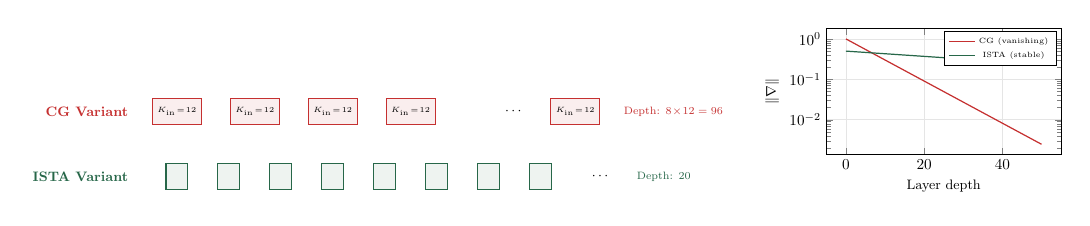
\begin{tikzpicture}[scale=0.55, transform shape,
    block/.style={rectangle, draw, minimum width=0.5cm, minimum height=0.6cm, font=\tiny},
    arr/.style={-{Stealth}, thick}]

  % CG variant
  \node[font=\small\bfseries, text=warningred, anchor=east] at (-1, 1.5) {CG Variant};
  \foreach \i in {0,...,3} {
    \node[block, draw=warningred, fill=warningred!8] (cg\i) at (\i*1.8, 1.5) {$K_{\text{in}}\!=\!12$};
  }
  \node at (7.8, 1.5) {\small$\cdots$};
  \node[block, draw=warningred, fill=warningred!8] (cg7) at (9.2, 1.5) {$K_{\text{in}}\!=\!12$};
  \node[right, font=\scriptsize, text=warningred] at (10.2, 1.5) {Depth: $8\!\times\!12=96$};

  % ISTA variant
  \node[font=\small\bfseries, text=forestgreen, anchor=east] at (-1, 0) {ISTA Variant};
  \foreach \i in {0,...,7} {
    \node[block, draw=forestgreen, fill=forestgreen!8] (is\i) at (\i*1.2, 0) {};
  }
  \node at (9.8, 0) {\small$\cdots$};
  \node[right, font=\scriptsize, text=forestgreen] at (10.5, 0) {Depth: $20$};

  % Gradient plot -- placed to the right
  \begin{scope}[xshift=15cm, yshift=0.5cm]
    \begin{axis}[
      width=7cm, height=4.5cm,
      xlabel={\small Layer depth},
      ylabel={\small $\|\nabla\|$},
      ymode=log,
      legend style={font=\tiny, at={(0.98,0.98)}, anchor=north east},
      grid=major,
      grid style={gray!20},
    ]
    \addplot[warningred, thick, domain=0:50, samples=50] {exp(-0.12*x)};
    \addlegendentry{CG (vanishing)}
    \addplot[forestgreen, thick, domain=0:50, samples=50] {0.5*exp(-0.015*x)};
    \addlegendentry{ISTA (stable)}
    \end{axis}
  \end{scope}
\end{tikzpicture}

\vspace{0.5em}
\begin{insightbox}
\centering
\textbf{Simpler layers $\times$ more layers $>$ Complex layers $\times$ fewer layers}
\end{insightbox}
\end{frame}

% =============================================
% SLIDE 12 — Full Architecture
% =============================================
\begin{frame}{Full Architecture}
\centering
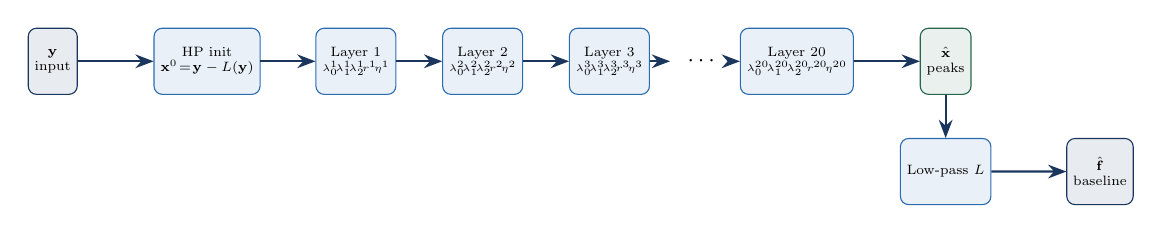
\begin{tikzpicture}[scale=0.7, transform shape,
    block/.style={rectangle, draw=steelblue, fill=steelblue!10, minimum height=1.2cm, rounded corners=3pt, align=center, font=\scriptsize},
    arr/.style={-{Stealth}, thick, navy}]

  % Input
  \node[block, draw=navy, fill=navy!10] (inp) at (0,0) {$\mathbf{y}$\\input};

  % High-pass init
  \node[block, minimum width=1.8cm] (init) at (2.8,0) {HP init\\$\mathbf{x}^0\!=\!\mathbf{y}-L(\mathbf{y})$};

  % Layers
  \node[block, minimum width=1.3cm] (l1) at (5.5,0) {Layer 1\\{\tiny $\lambda_0^1\!\lambda_1^1\!\lambda_2^1\!r^1\!\eta^1$}};
  \node[block, minimum width=1.3cm] (l2) at (7.8,0) {Layer 2\\{\tiny $\lambda_0^2\!\lambda_1^2\!\lambda_2^2\!r^2\!\eta^2$}};
  \node[block, minimum width=1.3cm] (l3) at (10.1,0) {Layer 3\\{\tiny $\lambda_0^3\!\lambda_1^3\!\lambda_2^3\!r^3\!\eta^3$}};
  \node[font=\large] at (11.8, 0) {$\cdots$};
  \node[block, minimum width=1.3cm] (lk) at (13.5,0) {Layer 20\\{\tiny $\lambda_0^{20}\!\lambda_1^{20}\!\lambda_2^{20}\!r^{20}\!\eta^{20}$}};

  % Peak output
  \node[block, draw=forestgreen, fill=forestgreen!10] (xout) at (16.2,0) {$\hat{\mathbf{x}}$\\peaks};

  % Baseline
  \node[block, draw=steelblue, fill=steelblue!10] (lp) at (16.2,-2) {Low-pass $L$};
  \node[block, draw=navy, fill=navy!10] (fout) at (19,-2) {$\hat{\mathbf{f}}$\\baseline};

  % Arrows
  \draw[arr] (inp) -- (init);
  \draw[arr] (init) -- (l1);
  \draw[arr] (l1) -- (l2);
  \draw[arr] (l2) -- (l3);
  \draw[arr] (l3) -- (11.2, 0);
  \draw[arr] (12.4, 0) -- (lk);
  \draw[arr] (lk) -- (xout);
  \draw[arr] (xout.south) -- ++(0,-0.5) -| (lp.north);
  \draw[arr] (lp) -- (fout);
\end{tikzpicture}

\vspace{1em}
\begin{tcolorbox}[colback=navy!5, colframe=navy, boxrule=0.5pt]
\centering
Signal length $N=4096$ \quad|\quad $K=20$ layers \quad|\quad 5 params/layer \quad|\quad \textbf{100 total learnable scalars}
\end{tcolorbox}
\end{frame}

% =============================================
% SLIDE 13 — The Development Timeline
% =============================================
\begin{frame}{The Development Timeline}
\note{Progressive development: each experiment adds one key idea. The sweet spot is in the middle.}
\centering
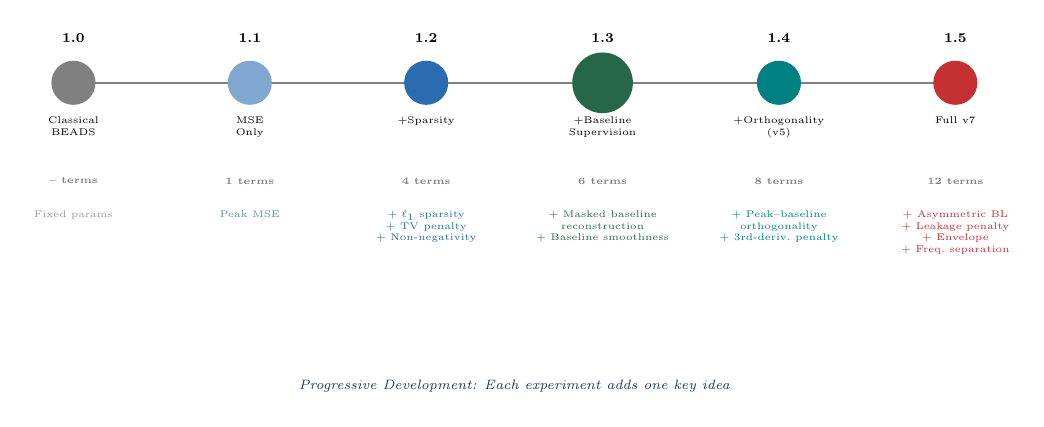
\begin{tikzpicture}[scale=0.7, transform shape]
  % Timeline line
  \draw[thick, gray] (0,0) -- (16,0);

  % Nodes
  \foreach \x/\lab/\sub/\col/\sz in {
    0/{1.0}/{Classical\\BEADS}/gray/0.4,
    3.2/{1.1}/{MSE\\Only}/steelblue!60/0.4,
    6.4/{1.2}/{+Sparsity}/steelblue/0.4,
    9.6/{1.3}/{+Baseline\\Supervision}/forestgreen/0.55,
    12.8/{1.4}/{+Orthogonality\\(v5)}/teal/0.4,
    16/{1.5}/{Full v7}/warningred/0.4
  } {
    \fill[\col] (\x, 0) circle (\sz);
    \node[above=0.6cm, align=center, font=\scriptsize\bfseries] at (\x, 0) {\lab};
    \node[below=0.5cm, align=center, font=\tiny] at (\x, 0) {\sub};
  }

  % Loss term counts
  \foreach \x/\n in {0/--,3.2/1,6.4/4,9.6/6,12.8/8,16/12} {
    \node[below=1.6cm, font=\tiny\bfseries, text=gray] at (\x, 0) {\n\ terms};
  }

  % Loss terms added at each step
  \node[below=2.2cm, align=center, font=\tiny, text=gray!80] at (0, 0)
    {Fixed params};
  \node[below=2.2cm, align=center, font=\tiny, text=steelblue!80] at (3.2, 0)
    {Peak MSE};
  \node[below=2.2cm, align=center, font=\tiny, text=steelblue] at (6.4, 0)
    {$+\;\ell_1$ sparsity\\$+$ TV penalty\\$+$ Non-negativity};
  \node[below=2.2cm, align=center, font=\tiny, text=forestgreen] at (9.6, 0)
    {$+$ Masked baseline\\reconstruction\\$+$ Baseline smoothness};
  \node[below=2.2cm, align=center, font=\tiny, text=teal] at (12.8, 0)
    {$+$ Peak--baseline\\orthogonality\\$+$ 3rd-deriv.\ penalty};
  \node[below=2.2cm, align=center, font=\tiny, text=warningred] at (16, 0)
    {$+$ Asymmetric BL\\$+$ Leakage penalty\\$+$ Envelope\\$+$ Freq.\ separation};

  \node[font=\scriptsize\itshape, text=navy] at (8, -5.5) {Progressive Development: Each experiment adds one key idea};
\end{tikzpicture}
\end{frame}

% =============================================
% SLIDE 14 — Three-Stage Curriculum Training
% =============================================
\begin{frame}{Three-Stage Curriculum Training}
\centering
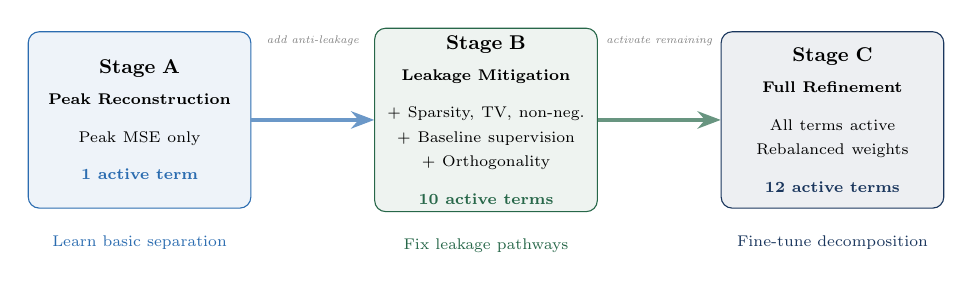
\begin{tikzpicture}[scale=0.8, transform shape,
    stage/.style={rectangle, rounded corners=4pt, minimum width=3.5cm, minimum height=2.8cm, align=center, font=\small, text width=3.3cm},
    arr/.style={-{Stealth}, very thick}]

  % Stage A
  \node[stage, draw=steelblue, fill=steelblue!8] (a) at (0, 0) {
    \textbf{Stage A}\\[3pt]
    {\scriptsize\textbf{Peak Reconstruction}}\\[6pt]
    {\scriptsize Peak MSE only}\\[6pt]
    {\scriptsize\textcolor{steelblue}{\textbf{1 active term}}}
  };

  % Stage B
  \node[stage, draw=forestgreen, fill=forestgreen!8] (b) at (5.5, 0) {
    \textbf{Stage B}\\[3pt]
    {\scriptsize\textbf{Leakage Mitigation}}\\[6pt]
    {\scriptsize $+$ Sparsity, TV, non-neg.}\\
    {\scriptsize $+$ Baseline supervision}\\
    {\scriptsize $+$ Orthogonality}\\[6pt]
    {\scriptsize\textcolor{forestgreen}{\textbf{10 active terms}}}
  };

  % Stage C
  \node[stage, draw=navy, fill=navy!8] (c) at (11, 0) {
    \textbf{Stage C}\\[3pt]
    {\scriptsize\textbf{Full Refinement}}\\[6pt]
    {\scriptsize All terms active}\\
    {\scriptsize Rebalanced weights}\\[6pt]
    {\scriptsize\textcolor{navy}{\textbf{12 active terms}}}
  };

  % Arrows with labels above, spaced away from boxes
  \draw[arr, steelblue!70] (a.east) -- (b.west);
  \node[above=0.15cm, font=\tiny\itshape, text=gray] at (2.75, 0.9) {add anti-leakage};

  \draw[arr, forestgreen!70] (b.east) -- (c.west);
  \node[above=0.15cm, font=\tiny\itshape, text=gray] at (8.25, 0.9) {activate remaining};

  % Labels below
  \node[below=0.3cm, font=\scriptsize, text=steelblue] at (a.south) {Learn basic separation};
  \node[below=0.3cm, font=\scriptsize, text=forestgreen] at (b.south) {Fix leakage pathways};
  \node[below=0.3cm, font=\scriptsize, text=navy] at (c.south) {Fine-tune decomposition};
\end{tikzpicture}

\vspace{0.8em}
\begin{insightbox}
\centering
\textbf{Why curriculum?} Activating 12 loss terms from scratch overwhelms 100 parameters.\\[3pt]
Stage A provides a stable initialization before anti-leakage penalties introduce competing gradients.
\end{insightbox}

\vspace{0.3em}
{\small\textcolor{forestgreen}{\textbf{Thesis model (v5):}} Stage A $\rightarrow$ Stage B only (8 terms). \quad
\textcolor{warningred}{\textbf{v7:}} All three stages (12 terms) --- performed worse.}
\end{frame}

% =============================================
% SLIDE 15 — Exp 1.0: Classical BEADS
% =============================================
\begin{frame}{Exp 1.0: Classical BEADS (Baseline)}
\begin{itemize}
  \item Apply classical BEADS with published default parameters
  \item Parameters designed for unnormalized data (amplitudes $\sim$100s)
  \item Applied to normalized $[0,1]$ test signals
\end{itemize}

\vspace{0.8em}
\begin{resultbad}
\centering
\begin{tabular}{lc}
\toprule
\textbf{Metric} & \textbf{Value} \\
\midrule
Area Error & \textbf{99.99\%} \\
Peak Correlation & 0.746 \\
Baseline Leakage Index & 0.837 \\
\bottomrule
\end{tabular}
\vspace{0.3em}

Almost all peak content treated as baseline.
\end{resultbad}

\vspace{0.5em}
\textbf{Takeaway:} Default parameters catastrophically fail on normalized data --- \textbf{the tuning problem in its most acute form}.
\end{frame}

% =============================================
% SLIDE 15 — Exp 1.1: Naive Unrolling
% =============================================
\begin{frame}{Exp 1.1: Naive Unrolling (MSE Only)}
Train with reconstruction loss only: $\alpha_{\text{mse}} = 1.0$, all others $= 0$.

\vspace{0.5em}
\centering
\begin{tabular}{lcc}
\toprule
\textbf{Metric} & \textbf{Classical} & \textbf{Exp 1.1} \\
\midrule
Peak MSE        & 21.27 & \textcolor{forestgreen}{\textbf{9.79}} \cmark \\
Peak Corr.      & 0.746 & 0.748 \\
Area Error      & 99.99\% & \textcolor{forestgreen}{\textbf{49.47\%}} \cmark \\
BLI             & 0.837 & \textcolor{forestgreen}{\textbf{0.593}} \cmark \\
Neg.\ Fraction  & 0.000 & \textcolor{warningred}{0.295} \xmark \\
\bottomrule
\end{tabular}

\vspace{0.8em}
\begin{insightbox}
\textbf{Algorithm unrolling works} --- but the architecture has an inherent sparsity bias.
\end{insightbox}
\end{frame}

% =============================================
% SLIDE 16 — Exp 1.2: + Sparsity Priors
% =============================================
\begin{frame}{Exp 1.2: + Sparsity Priors}
Add $\ell_1$ sparsity, total variation, non-negativity penalties.

\vspace{0.5em}
\begin{columns}[T]
\begin{column}{0.48\textwidth}
\begin{resultgood}
\textbf{Improved:}\\[3pt]
Peak Corr: 0.748 $\rightarrow$ \textbf{0.785} \cmark\\
Neg.\ Fraction: 0.295 $\rightarrow$ \textbf{0.216} \cmark
\end{resultgood}
\end{column}
\begin{column}{0.48\textwidth}
\begin{resultbad}
\textbf{Unchanged:}\\[3pt]
BLI: 0.593 $\rightarrow$ 0.597 \xmark\\
Area Error: 49.47\% $\rightarrow$ 49.51\% \xmark
\end{resultbad}
\end{column}
\end{columns}

\vspace{0.8em}
\begin{insightbox}
Sparsity priors improve peak \textit{shape} but do \textbf{NOT} address the leakage mechanism.
\end{insightbox}
\end{frame}

% =============================================
% SLIDE 17 — Exp 1.3: + Baseline Supervision
% =============================================
\begin{frame}{Exp 1.3: + Baseline Supervision}
Add masked baseline reconstruction + baseline smoothness.

\vspace{0.5em}
\centering
\begin{tabular}{lcc}
\toprule
\textbf{Metric} & \textbf{Exp 1.2} & \textbf{Exp 1.3} \\
\midrule
Peak MSE        & 9.79 & \textcolor{forestgreen}{\textbf{9.30}} \\
Peak Corr.      & 0.785 & \textcolor{forestgreen}{\textbf{0.793}} \\
Baseline MSE    & --- & 7.48 \\
\bottomrule
\end{tabular}

\vspace{0.8em}
\begin{resultgood}
\centering
\textbf{The single most impactful addition.}\\[3pt]
Direct gradient signal about baseline quality provides information\\that pure peak reconstruction cannot.
\end{resultgood}

\vspace{0.3em}
{\small Only 6 active loss terms.}
\end{frame}

% =============================================
% SLIDE 18 — Exp 1.4: + Orthogonality (v5)
% =============================================
\begin{frame}{Exp 1.4: + Orthogonality (v5 --- Thesis Model)}
Add peak--baseline orthogonality + baseline third-derivative penalty.

\vspace{0.5em}
\centering
\begin{tabular}{lcc}
\toprule
\textbf{Metric} & \textbf{Exp 1.3} & \textbf{Exp 1.4} \\
\midrule
Baseline MSE    & 7.48 & \textcolor{forestgreen}{\textbf{7.40}} \cmark \\
BLI             & 0.596 & \textcolor{forestgreen}{\textbf{0.592}} \cmark \\
Peak Corr.      & 0.793 & 0.785 {\scriptsize (mild decrease)} \\
\bottomrule
\end{tabular}

\vspace{0.8em}
\begin{insightbox}
Enforcing mutual exclusivity between peaks and baseline improves baseline quality at a mild cost to peak shape.
\end{insightbox}

\vspace{0.3em}
{\small \textbf{This is the thesis model configuration.}}
\end{frame}

% =============================================
% SLIDE 19 — Exp 1.5: Full Anti-Leakage Battery (v7)
% =============================================
\begin{frame}{Exp 1.5: Full Anti-Leakage Battery (v7)}
Activate \textbf{ALL 12 loss terms}: asymmetric baseline, leakage penalty, envelope constraint, frequency separation.

\vspace{0.5em}
\centering
\begin{tabular}{lcc}
\toprule
\textbf{Metric} & \textbf{Exp 1.4} & \textbf{Exp 1.5} \\
\midrule
Peak Corr.      & 0.785 & \textcolor{warningred}{\textbf{0.744}} \xmark \\
Peak MSE        & 9.36  & \textcolor{warningred}{\textbf{10.01}} \xmark \\
Neg.\ Fraction  & 0.211 & \textcolor{warningred}{\textbf{0.305}} \xmark \\
BLI             & 0.592 & \textcolor{warningred}{\textbf{0.611}} \xmark \\
\bottomrule
\end{tabular}

\vspace{0.8em}
\begin{resultbad}
\centering
\textbf{More loss terms $\neq$ better performance.}\\[3pt]
12 competing objectives overwhelm 100 parameters in 300 gradient steps.
\end{resultbad}
\end{frame}

% =============================================
% SLIDE 20 — The Over-Regularization Lesson
% =============================================
\begin{frame}{The Over-Regularization Lesson}
\centering
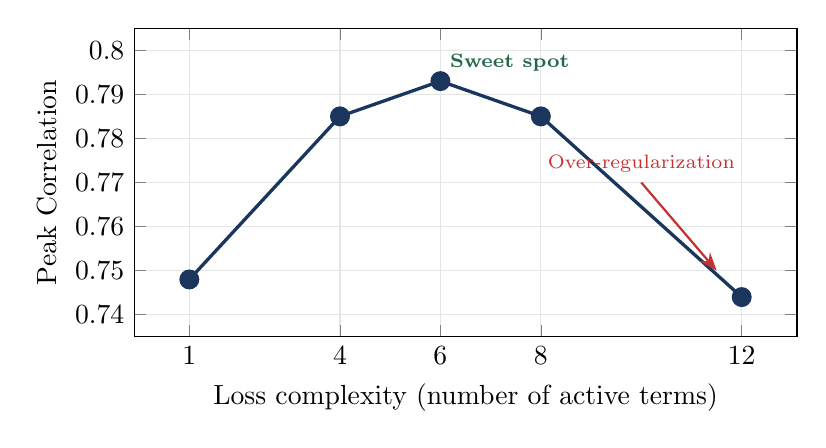
\begin{tikzpicture}
\begin{axis}[
  width=10cm, height=5.5cm,
  xlabel={Loss complexity (number of active terms)},
  ylabel={Peak Correlation},
  xtick={1,4,6,8,12},
  xticklabels={1,4,6,8,12},
  ytick={0.74,0.75,0.76,0.77,0.78,0.79,0.80},
  ymin=0.735, ymax=0.805,
  grid=major,
  grid style={gray!20},
  mark size=3pt,
]
\addplot[navy, very thick, mark=*] coordinates {
  (1, 0.748) (4, 0.785) (6, 0.793) (8, 0.785) (12, 0.744)
};
% Annotations
\node[above right, font=\scriptsize, text=forestgreen] at (axis cs:6, 0.793) {\textbf{Sweet spot}};
\draw[-{Stealth}, warningred, thick] (axis cs:10, 0.77) -- (axis cs:11.5, 0.75);
\node[above, font=\scriptsize, text=warningred] at (axis cs:10, 0.77) {Over-regularization};
\end{axis}
\end{tikzpicture}

\vspace{0.3em}
The relationship between loss complexity and model quality is \textbf{non-monotonic}.

{\small\textit{This motivated the 3-stage curriculum training strategy.}}
\end{frame}

% =============================================
% SLIDE 21 — The BLI Plateau
% =============================================
\begin{frame}{The BLI Plateau}
\note{This is the central negative result. The $\ell_1$ shrinkage is embedded in the forward computation. Loss terms can adjust parameters but cannot alter the architecture.}
\centering
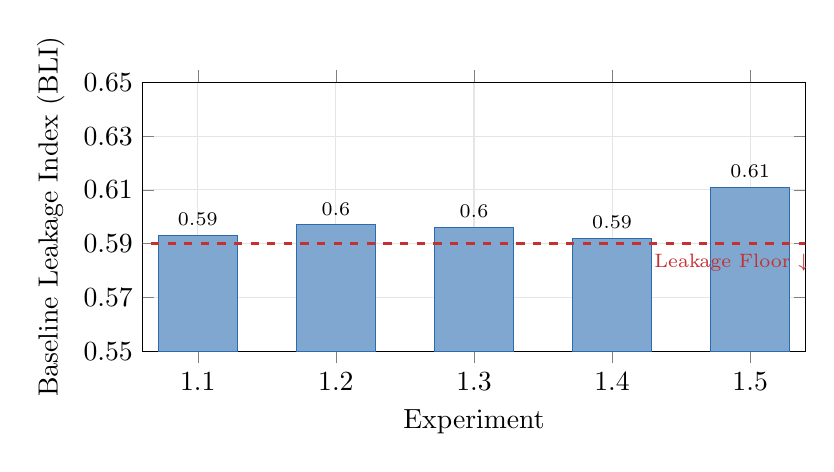
\begin{tikzpicture}
\begin{axis}[
  width=10cm, height=5cm,
  ybar,
  bar width=1cm,
  xlabel={Experiment},
  ylabel={Baseline Leakage Index (BLI)},
  xtick={1,2,3,4,5},
  xticklabels={1.1, 1.2, 1.3, 1.4, 1.5},
  ymin=0.55, ymax=0.65,
  ytick={0.55, 0.57, 0.59, 0.61, 0.63, 0.65},
  grid=major,
  grid style={gray!20},
  nodes near coords,
  every node near coord/.append style={font=\scriptsize},
]
\addplot[fill=steelblue!60, draw=steelblue] coordinates {
  (1, 0.593) (2, 0.597) (3, 0.596) (4, 0.592) (5, 0.611)
};
% Leakage floor line
\draw[warningred, dashed, very thick] (axis cs:0.3, 0.59) -- (axis cs:5.7, 0.59);
\node[font=\scriptsize, text=warningred, anchor=east] at (axis cs:5.5, 0.583) {Leakage Floor $\downarrow$};
\end{axis}
\end{tikzpicture}

\vspace{0.3em}
BLI varies by only \textbf{0.005} across Experiments 1.1--1.4.

\vspace{0.3em}
\begin{resultbad}
\centering
\textbf{Loss engineering cannot overcome the architectural inductive bias.}
\end{resultbad}
\end{frame}


% =============================================
% ACT III: THE DISCOVERY (Slides 22–28)
% =============================================
\section{Act III: The Discovery}

% =============================================
% SLIDE 22 — Why Leakage is Fundamental
% =============================================
\begin{frame}{Why Leakage is Fundamental}
\textbf{Soft-thresholding:}
\[
\mathcal{S}_\lambda(x) = \operatorname{sign}(x) \cdot \max\!\bigl(|x| - \lambda,\; 0\bigr)
\]

\centering
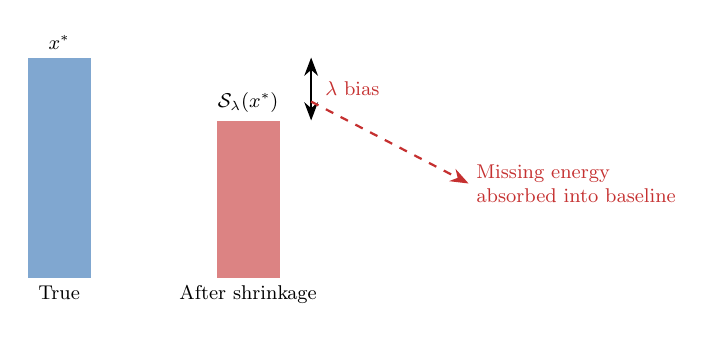
\begin{tikzpicture}[scale=0.8, transform shape]
  % True value bar
  \fill[steelblue!60] (0,0) rectangle (1, 3.5);
  \node[above, font=\small\bfseries] at (0.5, 3.5) {$x^*$};
  \node[below, font=\small] at (0.5, 0) {True};

  % Shrunk value bar
  \fill[warningred!60] (3,0) rectangle (4, 2.5);
  \node[above, font=\small\bfseries] at (3.5, 2.5) {$\mathcal{S}_\lambda(x^*)$};
  \node[below, font=\small] at (3.5, 0) {After shrinkage};

  % Shrinkage annotation
  \draw[{Stealth}-{Stealth}, thick] (4.5, 2.5) -- (4.5, 3.5);
  \node[right, font=\small, text=warningred] at (4.6, 3) {$\lambda$ bias};

  % Arrow to baseline
  \draw[-{Stealth}, thick, warningred, dashed] (4.5, 2.8) -- (7, 1.5);
  \node[right, font=\small, text=warningred, align=left] at (7, 1.5) {Missing energy\\absorbed into baseline};
\end{tikzpicture}

\vspace{0.5em}
For \textbf{any} $\lambda > 0$, every non-zero signal value is shrunk by exactly $\lambda$.

{\small In dense-peak regions where the sparsity assumption fails, this shrinkage accumulates across all peak samples.}
\end{frame}

% =============================================
% SLIDE 23 — Leakage in Action
% =============================================
\begin{frame}{Leakage in Action}
\centering
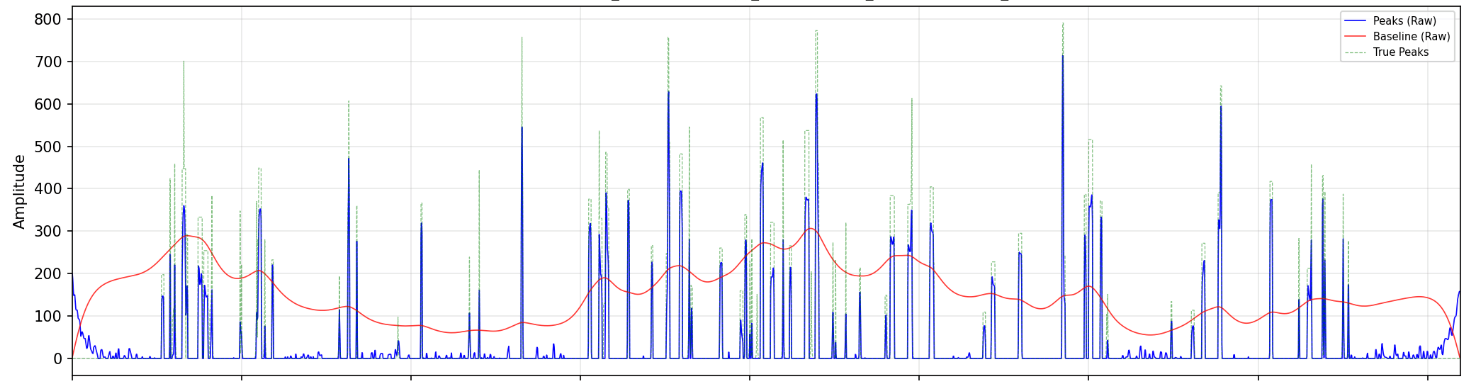
\includegraphics[width=0.9\textwidth, height=0.45\textheight, keepaspectratio]{figures/leakage-example.png}

\vspace{0.5em}
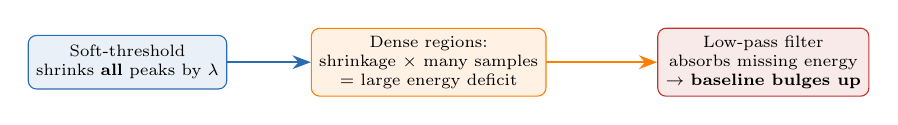
\begin{tikzpicture}[scale=0.85, transform shape,
    stepbox/.style={rectangle, rounded corners=3pt, minimum width=2.8cm, minimum height=0.8cm, align=center, font=\scriptsize},
    arr/.style={-{Stealth}, thick}]

  % Step 1
  \node[stepbox, draw=steelblue, fill=steelblue!10] (s1) at (0, 0)
    {Soft-threshold\\shrinks \textbf{all} peaks by $\lambda$};

  % Step 2
  \node[stepbox, draw=orange, fill=orange!10] (s2) at (4.5, 0)
    {Dense regions:\\shrinkage $\times$ many samples\\$=$ large energy deficit};

  % Step 3
  \node[stepbox, draw=warningred, fill=warningred!10] (s3) at (9.5, 0)
    {Low-pass filter\\absorbs missing energy\\$\rightarrow$ \textbf{baseline bulges up}};

  \draw[arr, steelblue] (s1) -- (s2);
  \draw[arr, orange] (s2) -- (s3);
\end{tikzpicture}

\vspace{0.5em}
\begin{resultbad}
\centering
\textcolor{forestgreen}{Green} = true peaks \quad \textcolor{blue}{Blue} = predicted peaks (shrunk) \quad \textcolor{warningred}{Red} = baseline (inflated)\\[3pt]
Where peaks are dense, the baseline \textbf{absorbs the energy} that soft-thresholding removes.
\end{resultbad}
\end{frame}

% =============================================
% SLIDE 24 — Raw Network Output Examples
% =============================================
\begin{frame}{Raw Network Output: Observed / Predicted / Ground Truth}
\centering
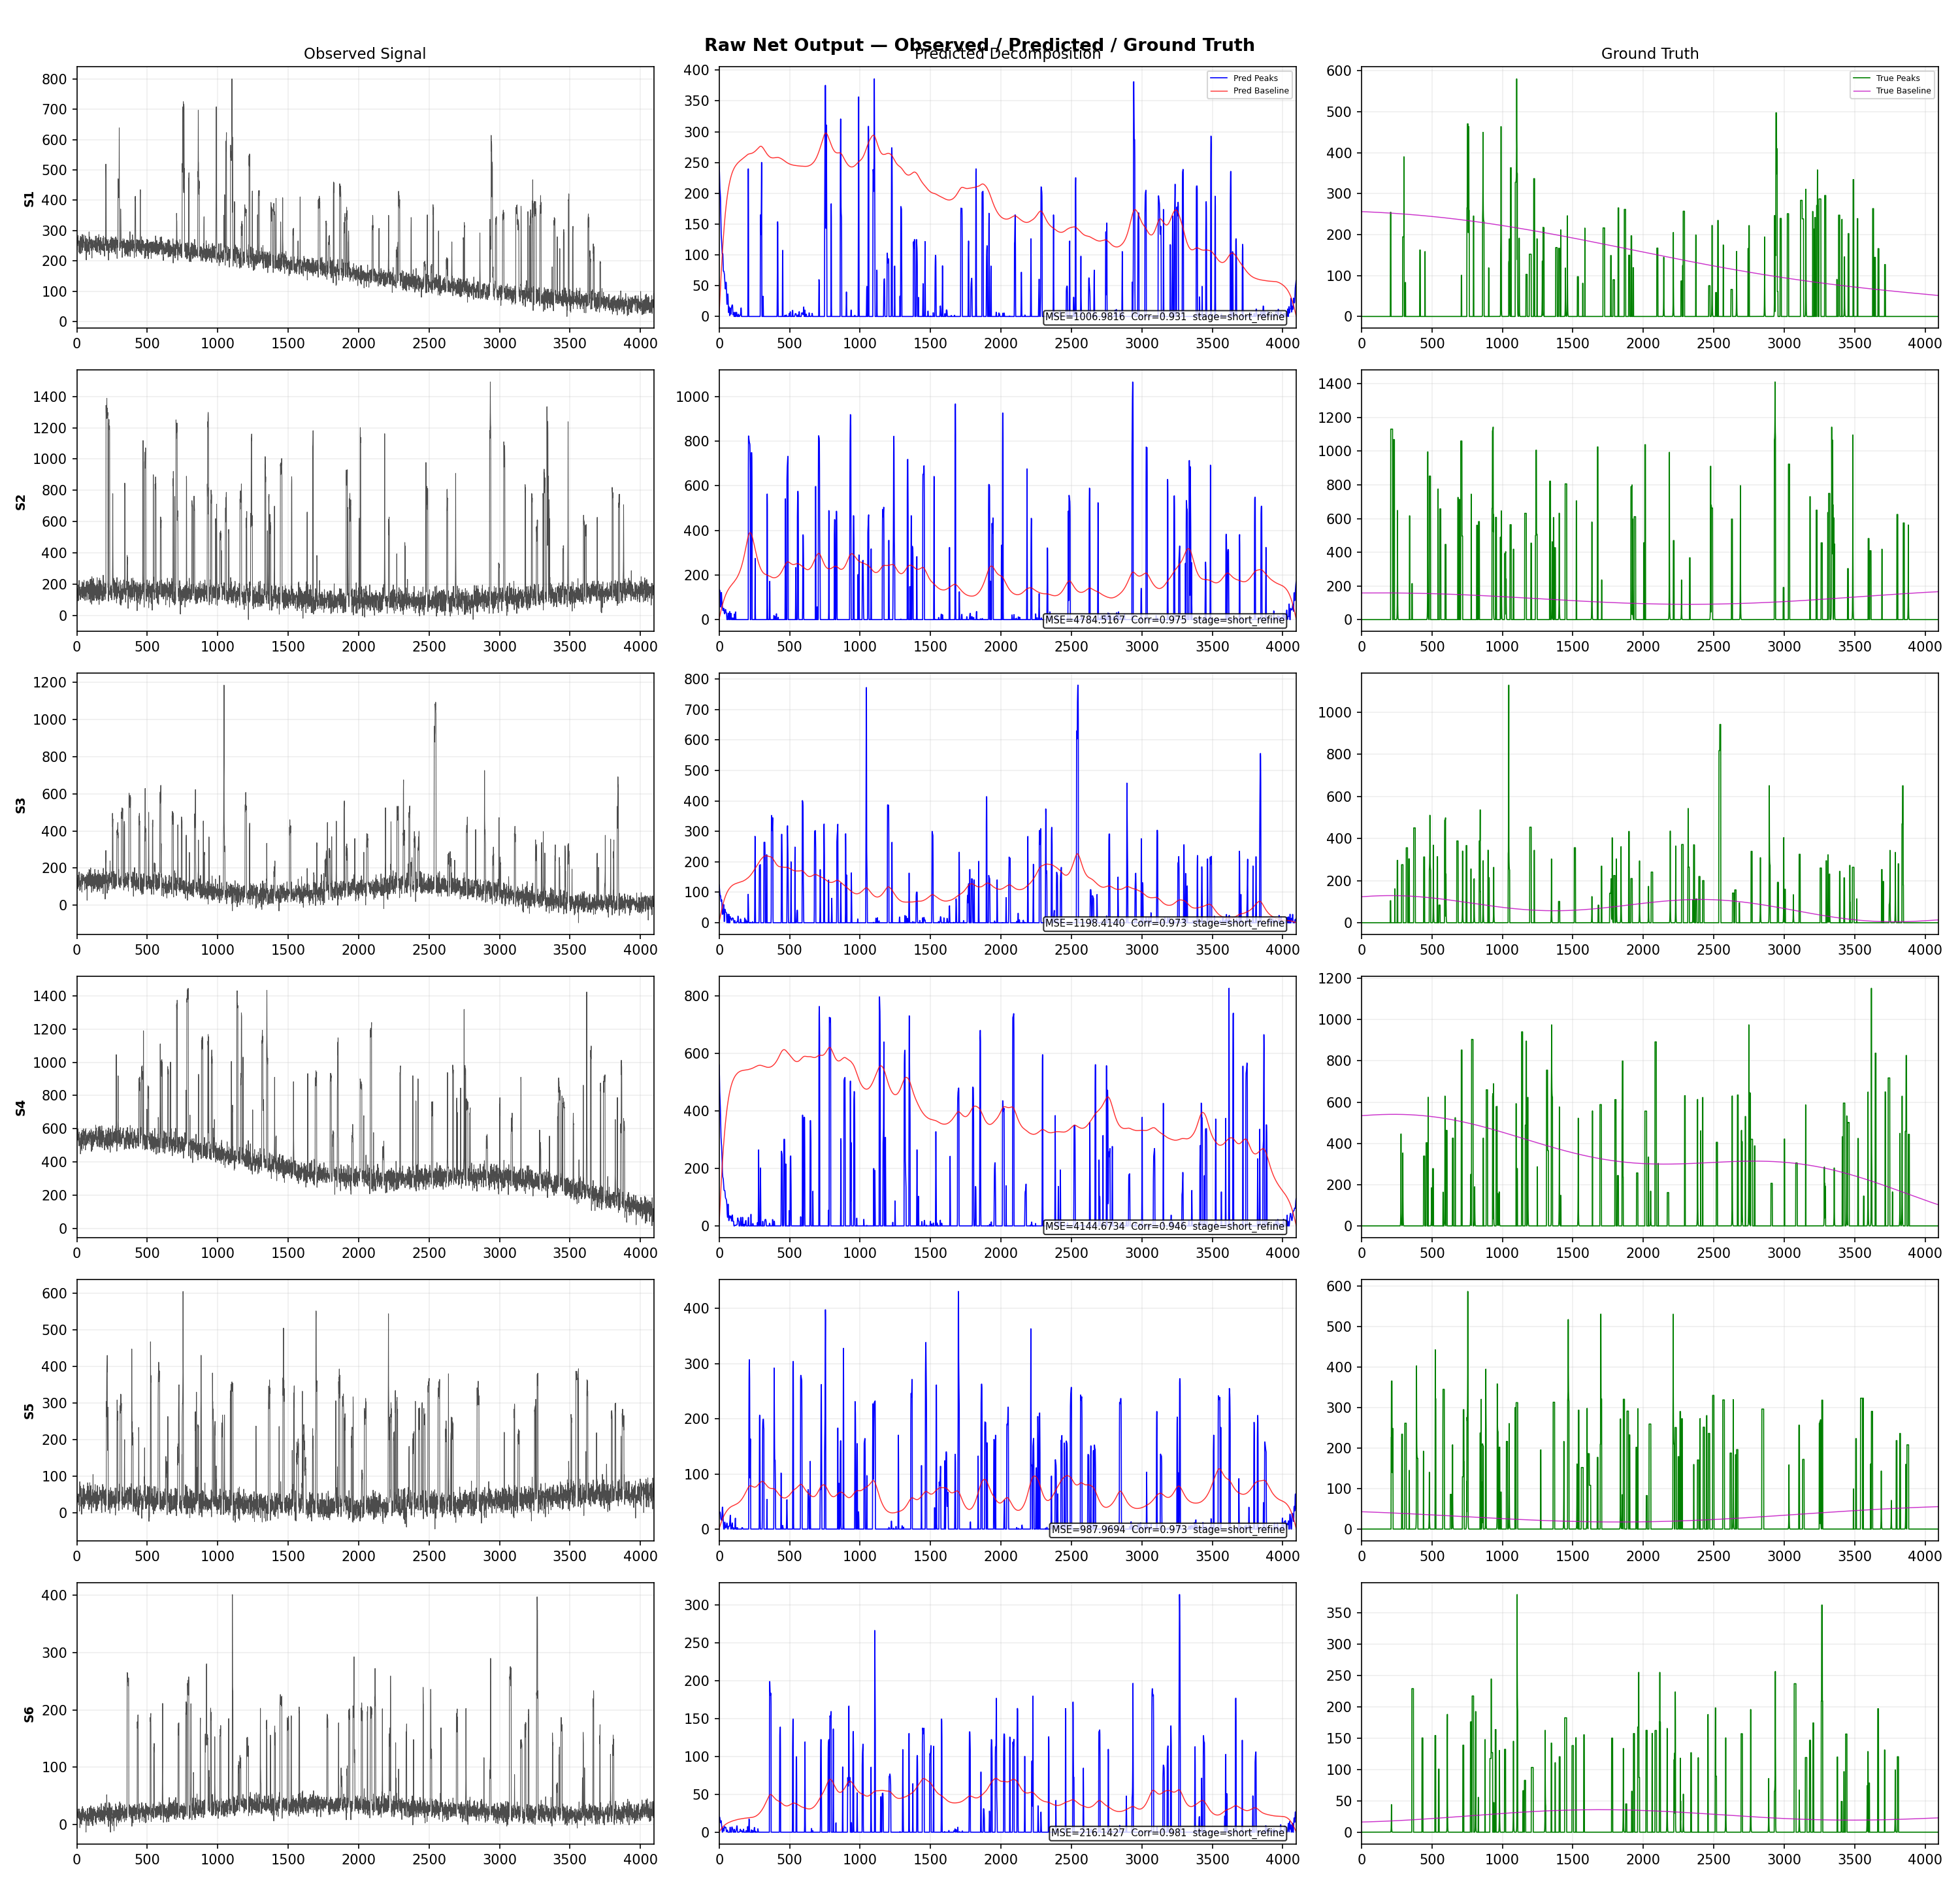
\includegraphics[width=\textwidth, height=0.85\textheight, keepaspectratio]{figures/leakage-example-again.png}
\end{frame}

% =============================================
% SLIDE 25 — Three Root Causes
% =============================================
\begin{frame}{Three Root Causes of Baseline Leakage}
\begin{columns}[T]
\begin{column}{0.31\textwidth}
\centering
\textcolor{steelblue}{\textbf{Sparsity Assumption\\Violation}}

\vspace{0.5em}
{\small
Dense peaks overlap $\rightarrow$ signal is NOT sparse\\[0.3em]
$\ell_1$ over-shrinks $\rightarrow$ energy leaks to baseline
}
\end{column}

\begin{column}{0.31\textwidth}
\centering
\textcolor{steelblue}{\textbf{Fixed Cutoff\\Frequency}}

\vspace{0.5em}
{\small
$f_c = 0.006$ for ALL signals\\[0.3em]
Broad peaks have energy below $f_c$ $\rightarrow$ attributed to baseline
}
\end{column}

\begin{column}{0.31\textwidth}
\centering
\textcolor{steelblue}{\textbf{Spatially Uniform\\Regularization}}

\vspace{0.5em}
{\small
Same $\lambda$ everywhere\\[0.3em]
Dense regions need weak $\lambda$,\\ sparse regions need strong $\lambda$
}
\end{column}
\end{columns}

\vspace{1em}
\begin{resultbad}
\centering
All three compound in \textbf{dense-peak regions} --- where accurate baseline correction is most needed.
\end{resultbad}
\end{frame}

% =============================================
% SLIDE 24 — Emergent Parameter Specialization
% =============================================
\begin{frame}{Emergent Parameter Specialization}
\centering
\begin{tabular}{lccc}
\toprule
\textbf{Parameter} & \textbf{Layer 0} & \textbf{Layer 3} & \textbf{Layer 5} \\
\midrule
$\lambda_0$ (sparsity)   & 0.481 & 1.198 & 2.000* \\
$r$ (asymmetry)           & 3.36  & 2.00* & 9.67 \\
$\eta$ (step size)        & 0.248 & 0.191 & 0.243 \\
\bottomrule
\end{tabular}

\vspace{0.8em}
\begin{itemize}
  \setlength\itemsep{0.4em}
  \item \textbf{Early layers}: gentle, conservative separation (low $\lambda_0$, moderate $r$)
  \item \textbf{Late layers}: aggressive refinement (high $\lambda_0$, strong asymmetry)
  \item \textbf{Step size}: determined by filter spectral properties, not layer position
\end{itemize}

\vspace{0.5em}
\begin{resultgood}
\centering
This specialization \textbf{emerges from training} --- all layers initialized identically.
\end{resultgood}
\end{frame}

% =============================================
% SLIDE 25 — What Actually Worked
% =============================================
\begin{frame}{What Actually Worked}
\begin{enumerate}
  \setlength\itemsep{0.7em}
  \item[\cmark] Algorithm unrolling eliminates per-signal tuning\\
    {\small ($2\times$ MSE improvement over default BEADS)}
  \item[\cmark] Masked baseline supervision is the single most impactful loss term
  \item[\wmark] Baseline leakage persists at BLI $\approx 0.59$ --- a fundamental $\ell_1$ limit
  \item[\xmark] More loss terms $\neq$ better: over-regularization degrades performance
  \item[\cmark] Learned parameters exhibit emergent layer specialization
\end{enumerate}

\vspace{0.8em}
\begin{insightbox}
\centering
The negative results (3, 4) are \textbf{as important as the positive ones}.
\end{insightbox}
\end{frame}

% =============================================
% SLIDE 26 — Fixing Leakage: The Peak Trade-Off
% =============================================
\begin{frame}{Fixing Leakage: The Peak Trade-Off}
\centering
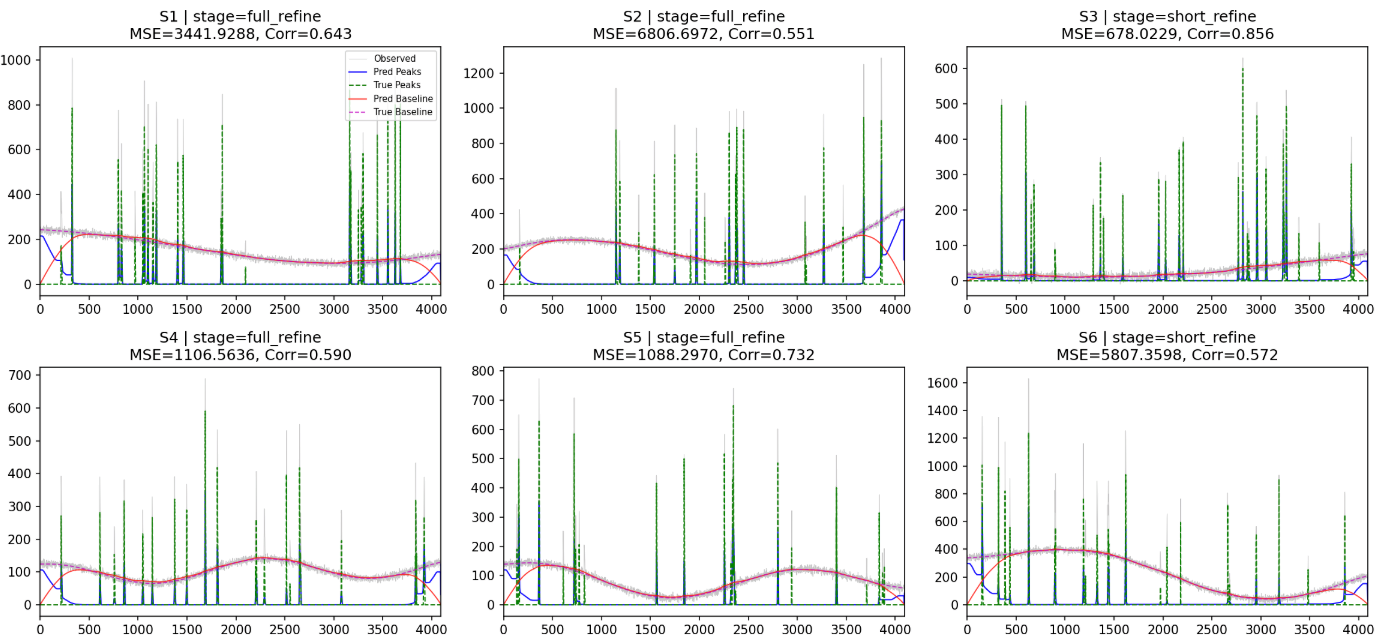
\includegraphics[width=0.95\textwidth, height=0.55\textheight, keepaspectratio]{figures/leakage-fix-example.png}

\vspace{0.3em}
{\small\textcolor{forestgreen}{\textbf{Baseline improves}} with anti-leakage terms, but \textcolor{warningred}{\textbf{peaks degrade}} --- the same penalties over-shrink peak amplitudes.}
\end{frame}

% =============================================
% SLIDE 27 — Limitations
% =============================================
\begin{frame}{Limitations}
\begin{itemize}
  \setlength\itemsep{0.5em}
  \item Quantitative evaluation on \textbf{synthetic data} --- real GC chromatographs tested qualitatively (visually plausible baselines, but no ground truth for metrics)
  \item No comparison with arPLS, airPLS, or deep learning baselines
  \item Dense $O(N^2)$ matrices --- 128\,MB per buffer at $N\!=\!4096$
  \item Fixed cutoff frequency $f_c$ (not learnable due to SciPy--PyTorch boundary)
  \item ${\sim}50\%$ area error on synthetic data --- not deployment-ready for quantitative analysis
\end{itemize}

\vspace{0.8em}
\begin{tcolorbox}[colback=gray!5, colframe=gray, boxrule=0.5pt]
\centering
This is a \textbf{methodological exploration} --- but the architecture is promising for real-world deployment.
\end{tcolorbox}
\end{frame}

% =============================================
% SLIDE 27 — Future Directions
% =============================================
\begin{frame}{Future Directions}
\begin{enumerate}
  \setlength\itemsep{0.6em}
  \item \textbf{Group sparsity ($\ell_{2,1}$ penalty)}\\
    {\small Replace element-wise $\ell_1$ with block soft-thresholding.\\
    Preserves within-group amplitudes $\rightarrow$ \textcolor{forestgreen}{directly addresses leakage.}}

  \item \textbf{Banded matrix implementation in PyTorch}\\
    {\small $O(N^2) \rightarrow O(N \cdot b)$.\quad Enables $N = 100{,}000+$ signals natively on GPU.}

  \item \textbf{Real chromatographic validation}\\
    {\small Spike-and-recovery experiments, consensus labeling with expert chromatographers.\\
    \textcolor{warningred}{The critical missing piece for deployment.}}

  \item \textbf{Edge deployment on STM32 microcontrollers}\\
    {\small Only \textbf{100 scalar parameters} + banded ops $\rightarrow$ tiny memory footprint.\\
    At $N\!=\!4096$ with banded matrices: ${\sim}$200\,KB RAM (signal buffers + filter bands).\\
    Feasible on STM32H7-class MCUs (1\,MB+ SRAM, Cortex-M7 @ 480\,MHz).\\
    \textcolor{forestgreen}{Enables real-time baseline correction on portable instruments.}}
\end{enumerate}
\end{frame}

% =============================================
% SLIDE 28 — Thank You
% =============================================
\begin{frame}[standout]
  \Large Thank You

  \vspace{1em}
  \normalsize
  Algorithm unrolling bridges interpretability and generalization ---\\
  and reveals the fundamental limits of sparsity-based signal decomposition.

  \vspace{1.5em}
  \small
  Advisor: Professor Ivan Selesnick\\[0.3em]
  Saad Zubairi --- NYU Tandon --- May 2026

  \vspace{1.5em}
  \Large Questions?
\end{frame}

\end{document}
